% This file was created with tikzplotlib v0.9.17.
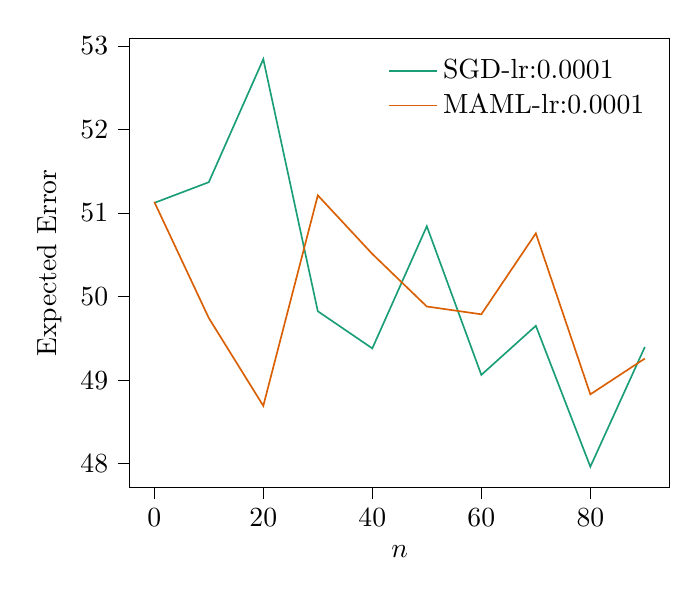
\begin{tikzpicture}

\definecolor{color0}{rgb}{0.105882352941176,0.619607843137255,0.466666666666667}
\definecolor{color1}{rgb}{0.850980392156863,0.372549019607843,0.00784313725490196}

\begin{axis}[
legend cell align={left},
legend style={fill opacity=0.8, draw opacity=1, text opacity=1, draw=none},
tick align=outside,
tick pos=left,
x grid style={white!69.0196078431373!black},
xlabel={\(\displaystyle n\)},
xmin=-4.5, xmax=94.5,
xtick style={color=black},
y grid style={white!69.0196078431373!black},
ylabel={Expected Error},
ymin=47.7199107347417, ymax=53.0842353498106,
ytick style={color=black}
]
\addplot [semithick, color0]
table {%
0 51.1202454390532
10 51.3681716366622
20 52.840402412762
30 49.8240947436692
40 49.3796294861132
50 50.8412107221978
60 49.0623684624619
70 49.6501556550569
80 47.9637436717903
90 49.3965065319105
};
\addlegendentry{SGD-lr:0.0001}
\addplot [semithick, color1]
table {%
0 51.133041350814
10 49.7432961071916
20 48.6919962214245
30 51.2106849654085
40 50.5096121950441
50 49.8805843737812
60 49.787605354798
70 50.7562072134105
80 48.8300028865188
90 49.2581008945567
};
\addlegendentry{MAML-lr:0.0001}
\end{axis}

\end{tikzpicture}
